\documentclass[12pt,a4paper]{report}
\usepackage[utf8]{inputenc}
\usepackage{amsmath}
\usepackage{amsfonts}
\usepackage{amssymb}
\usepackage{graphicx}
\usepackage{multicol}
\usepackage{changepage}
\usepackage{float}
\usepackage{cite}
\usepackage{url}

\usepackage[left=2cm,right=2cm,top=2cm,bottom=2cm]{geometry}
\author{Hernández Luis Sergio Ángel}
\begin{document}
%encabezado 
\pagestyle{plain}{
\pagestyle{empty}
\noindent

{\small
\begin{tabular}{p{0.626\textwidth} p{0.626\textwidth} }

\includegraphics[scale=0.7]{unam.png} &  
\includegraphics[scale=0.15]{fi.png}
\end{tabular}
}

%datos de la caratula
\begin{center}
\par\vspace{2cm} %Rspacoo dejado antes del encabezado
{
\Huge\textbf{
Universidad Nacional Autónoma de México \\[2cm] Facultad de Ingeniería
}
}
\par\vspace{1 cm}
{
\Large\textbf{ Materia: Programación Orientada a Objetos \\ Profesor: Edgar Tista García \\ Grupo: 03
}
}
\par\vspace{1cm}
{
\large\textbf{Nombres: Félix Flores Paul Jaime \\ Hernández Luis Sergio Ángel \\ Ricardo Alonso Velasco Vanegas } 
}
\par\vspace{1 cm}
{
\large\textbf{Fecha: 21 de mayo de 2019 } 
}
\par\vspace{3cm}
\end{center}
\clearpage
\section*{Objetivos}

Que el alumno ponga en práctica todos los conceptos vistos a lo largo del curso en una aplicación real.

Que el alumno fortalezca sus habilidades la programación orientada a objetos.

Que el alumno fortalezca sus habilidades en trabajo en equipo.
\section*{Introducción}
La programación orientada a objetos es una “filosofía”, un modelo de programación, con su teoría y su metodología, que conviene conocer y estudiar antes de nada. Un lenguaje orientado a objetos es un lenguaje de programación que permite el diseño de aplicaciones orientadas a objetos.

Las estructuras de datos representan formas de almacenar conjuntos de datos del mismo tipo. Además, deben deben proveer mecanismos de acceso rápido, ágiles y eficientes. Estas estructuras son pieza fundamental de los algoritmos y la elección de dicha estructura permite la facilidad en la construcción de estos. Por lo contrario, si la estructura elegida no es la indicada para la construcción del algoritmo, entonces su desarrollo se tornará más complejo hasta el punto de ser imposible su construcción.

Con esto en mente se presentará a continuación las principales estructuras de datos, así como su funcionamiento y operaciones principales de manera teórica, y ya abordado los fundamentos de estas, se comentará su implementación y estructura dentro del lenguaje de programación Java.

\section*{Colecciones}
Ya conociendo algunos de los tipos de estructuras más utilizados en el ámbito de la programación y su importancia Java nos proporciona una implementación de dichas estructuras en este lenguaje las cuales, además de proporcionar las operaciones básicas que se requieren para su manejo, ofrece un conjunto de métodos que facilitan el trabajo con estas mismas. 
\subsection*{Jerarquía de colecciones}
Antes de iniciar con el estudio sobre la estructura con la cual se conforma este conjunto de herramientas iniciamos por definir que es una clase y una interfaz.

Una clase es la descripción de un conjunto de objetos iguales. En otras palabras se podría considerar como una plantilla de la cual se pueden crear un conjunto infinito de objetos iguales.

Una interfaz es un conjunto de constantes y métodos abstractos (métodos los cuales no contienen sentencias, instrucciones o variables y deben ser sobrescritos por las clases que los heredan) con el fin de permitir la herencia múltiple dentro del lenguaje.  

Con esto aclarado, ya que estos conceptos no deben de confundirse unos con otros, iniciemos con la definición de una colección.

Una colección es una estructura de datos que puede guardar referencias del tipo de objeto del cual se compondrá la colección (Esto se define con anterioridad en la creación de esta).

Como nos pudimos dar cuenta hay operaciones que implementan todas las estructuras de datos ya sean lineales o no lineales, como por ejemplo el agregar o eliminar un elemento, pero también hay operaciones que comparten únicamente un conjunto de estructuras ya que su forma de operar es semejante o una es una reimplementación de otra como podría ser las listas simplemente ligadas y las doblemente ligadas. Con esto en mente Java creo interfaces las cuales declaran las operaciones que deben de realizar de forma genérica en varios tipos de colecciones.
\begin{figure}[hbtp]
\centering
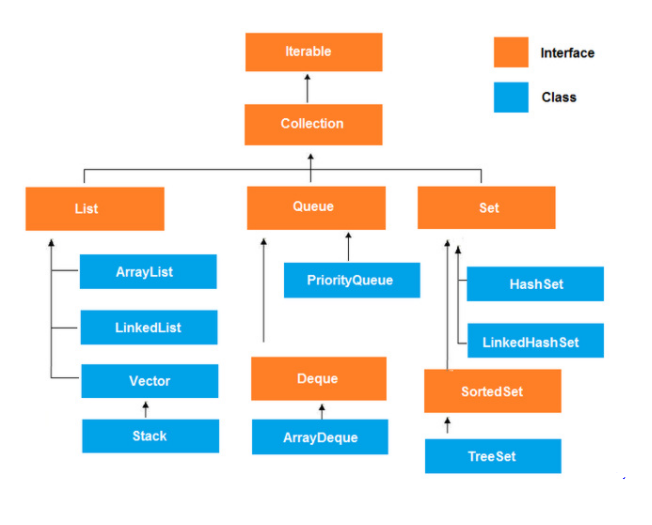
\includegraphics[scale=0.5]{colecciones.PNG}
\end{figure}

Las clases e interfaces  se encuentran en los paquetes java.util y java.util.concurrent.

Como podemos apreciar, la raíz de la jerarquía de colecciones es la interfaz Collection<E>. De entre las interfaces que extienden Collection<E> las más interesantes son List<E>, Set<E> y Queue<E> que definen, respectivamente, listas, conjuntos y colas. En versiones anteriores de Java las colecciones trabajaban con referencias del tipo Object ya que todas las clases heredan de manera implícita o explícita de esta, pero en la mayoría de los casos las colecciones deben de trabajar con tipos de objetos específico y por lo tanto se debía de realizar una conversión al tipo de objeto apropiado.

Para eliminar este problema se mejoraron las colecciones con la implementación de las herramientas de genéricos. Los genéricos nos permiten especificar el tipo exacto que se almacenará en una colección y nos da el  beneficio de la comprobación de tipos en tiempo de ejecución.   
  
Para una mayor comprensión de cuál es el objetivo de crear estas interfaces a continuación se muestra un breve resumen de las características que contienen  las clases que implementan cada interfaz.
\begin{figure}[hbtp]
\centering
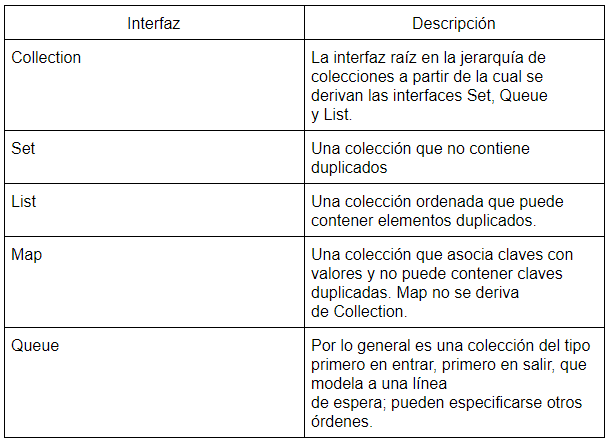
\includegraphics[scale=1]{tabla.PNG}
\end{figure}

\begin{figure}[hbtp]
\caption{Diagrama de decisión para el uso de colecciones}
\centering
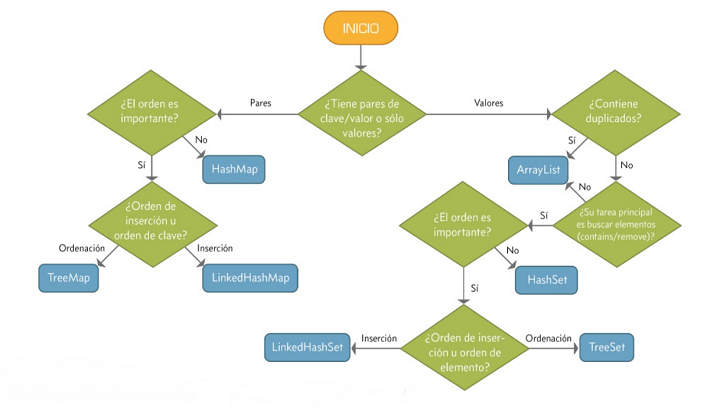
\includegraphics[scale=0.6]{java.png}
\end{figure}
Un punto importante a notar es el hecho de que las colecciones trabajan únicamente con objetos. Esto en un inicio se pensaría cómo inconveniente si se desearan colecciones de tipos de dato primitivos pero, si recordamos a las clases envolventes, este hecho es más bien una ventaja ya que los envolventes poseen un gran conjunto de métodos útiles para analizar una colección. 

\section*{Interfaz Collection y la clase Collections}
Dentro de las colecciones se encuentran los métodos básicos e indispensables para toda estructura de datos como el añadir o eliminar elementos  además de operaciones de gran utilidad pero no vitales como la búsqueda y el ordenamiento. Los primeros tipos de métodos varían dependiendo de la estructura y por lo tanto requieren una implementación diferente en cada caso, pero en el caso de la búsqueda por ejemplo se puede aplicar a cada estructura de manera igual sin temor a que ocurran incongruencias. Con esto en mente Java creo la interfaz Collection y la clase Collections.

La interfaz Collection contiene operaciones masivas (es decir, operaciones que se llevan a cabo en toda una colección) como lo son agregar, borrar y comparar objetos además de proporcionar un método que retorna un objeto Iterator, el cual permite a un programa recorrer la colección y eliminar elementos de la misma durante la iteración.

La clase Collections proporciona métodos estáticos (static) encargados de la búsqueda y ordenación. Más adelante se abordarán más a fondo estos métodos.

Durante el camino que uno toma para aprender a programar, ya sea en cualquier lenguaje, se ha tenido que abordar el tema de los arreglos. Como ya se sabe un arreglo es un conjunto de información del mismo tipo la cual se puede acceder a dicha información de manera arbitraria sabiendo la posición que ocupa el elemento de interés (recordemos que un arreglo inicia desde la posición 0).

Uno de los mayores problemas de un arreglo es la inserción de nuevos elementos ya que para hacerlo se debía de crear un nuevo arreglo y copiar el contenido existente más el que se desea agregar dentro del nuevo y esto se repite en cada nuevo elemento.

La clase collection soluciono este problema con el apoyo de la interfaz list, la cual permite la inserción dinámica de elementos

\section*{Interfaz List}
Esta interfaz tiene como principales características el poder acceder a sus elementos en base a su índice y también permite el ingreso de elementos repetidos. Proporciona más de un método con el cual poder ingresar elementos en base a su índice.

Esta interfaz proporciona un objeto de la clase IteratorList que permite el recorrido de elementos dentro de cualquier objeto que implemente List.

Dependiendo del tipo de colección que implemente a List se puede permitir la inclusión de elementos nulos (null) o incluso restringir el tipo de objeto que almacena.

\section*{ArrayList}
Como se ha comentado antes el mayor problema al momento de trabajar con arreglos es el redimensionar su tamaño, ya sea aumentandolo o disminuyendolo.  La clase de colección ArrayList (perteneciente a java.util) provee una solución conveniente a este problema, ya que puede cambiar su tamaño de forma dinámica para dar más cabida a elementos. 
Esta clase implementa la interfaz list (es decir, se acceden a los elementos en base a su índice) junto con todas sus operaciones y aceptando valores nulos. En pocas palabras, la clase ArrayList es una representación dinámica de los arreglos  y por lo tanto tiene un límite para el almacenamiento de valores, esto se explica debido a que solo se pueden acceder en base a un índice, el cual es un número entero, por lo tanto su valor límite está indicado por el valor entero más alto.

\subsection*{Métodos de ArrayList }
boolean add(E e): Anexa el elemento especificado al final de esta lista.

void add(int index, E element): Inserta el elemento especificado en la posición especificada en esta lista.

boolean addAll(Collection<? extends E> c): Anexa todos los elementos de la colección especificada al final de esta lista, en el orden en que son devueltos por el iterador de la colección especificada.

boolean addAll(int index, Collection<? extends E> c): Inserta todos los elementos de la colección especificada en esta lista, comenzando en la posición especificada.

void clear(): Remueve todos los elementos de la lista.

Object clone(): Devuelve una copia superficial de esta instancia de ArrayList.

boolean contains(Object o): Devuelve verdadero si esta lista contiene el elemento especificado.

void ensureCapacity(int minCapacity): Aumenta la capacidad de esta instancia de ArrayList, si es necesario, para garantizar que pueda contener al menos el número de elementos especificado por el argumento de capacidad mínima.

void forEach(Consumer<? super E> action): Realiza la acción dada para cada elemento del Iterable hasta que todos los elementos hayan sido procesados o la acción arroje una excepción.

E get(int index): Devuelve el elemento en la posición especificada en esta lista.

int indexOf(Object o): Devuelve el índice de la primera aparición del elemento especificado en esta lista, o -1 si esta lista no contiene el elemento.

boolean isEmpty(): Devuelve verdadero si esta lista no contiene elementos.

\section*{LinkedList}
Lista enlazada son estructuras de datos lineales donde los elementos no se almacenan en ubicaciones contiguas y cada elemento es un objeto separado con una parte de datos y una parte de dirección. Los elementos están vinculados mediante punteros y direcciones. Cada elemento es conocido como un nodo. Debido a la dinamismo y la facilidad de las inserciones y eliminaciones, se prefieren a las matrices. También tiene algunas desventajas, ya que no se puede acceder directamente a los nodos, sino que debemos comenzar desde la cabeza y seguir el enlace para llegar a un nodo al que deseamos acceder.
Para almacenar los elementos en una lista enlazada usamos una lista doblemente enlazada que proporciona una estructura de datos lineal y también se usa para heredar una clase abstracta e implementar listas de listas e interfaces deque.

En Java, la clase LinkedList implementa la interfaz de lista. La clase LinkedList también consta de varios constructores y métodos como otras colecciones Java.

\subsection*{Métodos para LinkedList}
add (int index, E element): este método inserta el elemento especificado en la posición especificada en esta lista.

add(E e): este método agrega el elemento especificado al final de esta lista.

addAll (índice int, Colección c): este método inserta todos los elementos de la colección especificada en esta lista, comenzando en la posición especificada.

addAll (Colección c): este método Anexa todos los elementos de la colección especificada al final de esta lista, en el orden en que son devueltos por el iterador de la colección especificada.

addFirst (E e): este método inserta el elemento especificado al principio de esta lista.
addLast (E e): este método agrega el elemento especificado al final de esta lista.

clear (): este método elimina todos los elementos de esta lista.

clone (): este método devuelve una copia superficial de este LinkedList.

contains (Objeto o): este método devuelve verdadero si esta lista contiene el elemento especificado.

descendingIterator (): este método devuelve un iterador sobre los elementos en este deque en orden secuencial inverso.

element (): este método recupera, pero no elimina, el encabezado (primer elemento) de esta lista.

get (int index): este método devuelve el elemento en la posición especificada en esta lista.

getFirst (): este método devuelve el primer elemento de esta lista.

getLast (): este método devuelve el último elemento de esta lista.

indexOf (Objeto o): este método devuelve el índice de la primera aparición del elemento especificado en esta lista, o -1 si esta lista no contiene el elemento.

lastIndexOf (Object o): este método devuelve el índice de la última aparición del elemento especificado en esta lista, o -1 si esta lista no contiene el elemento.

listIterator (índice int): este método devuelve un iterador de lista de los elementos de esta lista (en la secuencia adecuada), comenzando en la posición especificada en la lista.

offer (E e): este método agrega el elemento especificado como la cola (último elemento) de esta lista.

offerFirst (E e): este método inserta el elemento especificado al principio de esta lista.

offerLast (E e): este método inserta el elemento especificado al final de esta lista.

peek (): este método recupera, pero no elimina, el encabezado (primer elemento) de esta lista.

peekFirst (): este método recupera, pero no elimina, el primer elemento de esta lista, o devuelve nulo si esta lista está vacía.

peekLast (): este método recupera, pero no elimina, el último elemento de esta lista, o devuelve nulo si esta lista está vacía.

poll (): este método recupera y elimina la cabecera (primer elemento) de esta lista.

pollFirst (): este método recupera y elimina el primer elemento de esta lista, o devuelve nulo si esta lista está vacía.

pollLast (): este método recupera y elimina el último elemento de esta lista, o devuelve nulo si esta lista está vacía.

pop (): este método hace saltar un elemento de la pila representada por esta lista.

push (E e): este método empuja un elemento en la pila representada por esta lista.

remove (): este método recupera y elimina el encabezado (primer elemento) de esta lista.

remove (int index): este método elimina el elemento en la posición especificada en esta lista.

remove (Objeto o): este método elimina la primera aparición del elemento especificado de esta lista, si está presente.

removeFirst (): este método elimina y devuelve el primer elemento de esta lista.

removeFirstOccurrence (Objeto o): este método elimina la primera aparición del elemento especificado en esta lista (cuando se atraviesa la lista de principio a fin).

removeLast (): este método elimina y devuelve el último elemento de esta lista.

removeLastOccurrence (Objeto o): este método elimina la última aparición del elemento especificado en esta lista (cuando se atraviesa la lista de principio a fin).

set (int index, E element): este método reemplaza el elemento en la posición especificada en esta lista con el elemento especificado.

size (): este método devuelve el número de elementos en esta lista.

spliterator (): este método crea un Spliterator de enlace tardío y rápido en todos los elementos de esta lista.

toArray (): este método devuelve una matriz que contiene todos los elementos de esta lista en la secuencia correcta (del primer al último elemento).

toArray (T [] a): este método devuelve una matriz que contiene todos los elementos de esta lista en la secuencia correcta (del primer al último elemento); el tipo de tiempo de ejecución de la matriz devuelta es el de la matriz especificada.

\section{Vector}
Los arrays en Java son suficientes para guardar tipos básicos de datos, y objetos de una determinada clase cuyo número conocemos de antemano. Algunas veces deseamos guardar objetos en un array pero no sabemos cuantos objetos vamos a guardar. Una solución es la de crear un array cuya dimensión sea más grande que el número de elementos que necesitamos guardar. La clase Vector nos proporciona una solución alternativa a este problema. Un vector es similar a un array, la diferencia estriba en que un vector crece automáticamente cuando alcanza la dimensión inicial máxima. Además, proporciona métodos adicionales para añadir, eliminar elementos, e insertar elementos entre otros dos existentes.

\begin{figure}[hbtp]
\centering
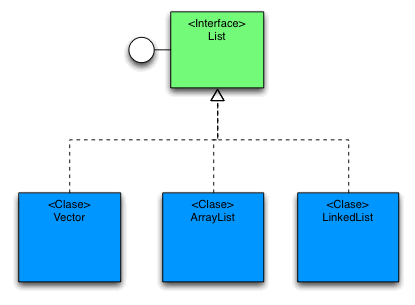
\includegraphics[scale=1]{interfazlist.PNG}
\end{figure}

\section*{Interfaz Set}
Esta interfaz tiene una peculiaridad, y es que no admite duplicados y es especialmente útil para ir almacenando datos sin la preocupación de que alguno se repita. Estos elementos o datos pueden estar ordenados o no.

Esta Interfaz, al igual que List, nos proporciona métodos para:

Añadir un elemento a la colección

Eliminar un elemento de la colección

Obtener un elemento de la colección

localizar un elemento en la colección

Iterar sobre la colección.
\subsection*{HashSet}
Representa un conjunto de valores únicos sin ordenar, no puede tener valores duplicados. Tiene una iteración más rápida que ArrayList, por lo tanto si queremos tener un conjunto de elementos únicos sin importarnos si están ordenados o no, está es nuestra elección.
Para construir un HashSet hacemos:

HashSet nomVariable=new HashSet();
\subsubsection*{Métodos más comunes}
Los métodos más comunes de esta colección son:

boolean add(object o): Añade un nuevo objeto a la colección, devolviendo true si lo ha insertado y false si no ha podido.

hs.add(new Integer(1)); Las colecciones no admiten tipos primitivos, con lo que deberemos envolver el tipo con la clase específica.

object remove(int posicion): Elimina de la colección el objeto la posición indicada. no hay que hacerle conversión de tipo, ya que, como lo a a eliminar, no le hace falta saber de que tipo es.
		hs.remove(0);
		
void clear(): Elimina todos los elementos almacenados en la colección.
		hs.clear();
int Size(): Devuelve el tamaño de la colección. 
		hs.size();
object clone(): Metodo que devuelve una copia del HashSet:
		HashSet newHs =new HashSet();
		newHs=(HashSet) hs.clone();
		 
boolean contains(object o): Método que devuelve true si la colección contiene el elemento pasado por parámetro.
		hs.contains(new Integer(1));

boolean isEmpty(): Método que devuelve true si la colección esta vacía.
		hs.isEmpty();
		
Iterator iterator(): Método que recorre los elementos de una colección.
Este tipo de colección no contiene un método get() para obtener los elementos de una colección, como List. En cambio, posee este método, el cual, combinado con un bucle while, nos permitirá ir recorriendo nuestra colección:
Iterator it=hs.iterator();

while(it.hasNext()){
System.out.println(it.next());
}
Bien, aquí lo que hacemos es, instanciar la interfaz Iterator, posteriormente utilizamos el método booleano "hasNext()" para indicarle al Iterator que mientras haya elementos en la colección siga recorriendola, y finalmente imprimimos por pantalla el elemento en el que este posicionado con el método "next()".

\subsection*{LinkedHashSet}
Esta colección es ordenada pero no clasificada, esto quiere decir que el orden de los elementos, es el mismo que el orden en el que se insertan. Ello conlleva una gran diferencia con HashSet, ya que esta no era ordenada. También hay que tener en cuenta que al ser ordenada tiene una iteración más lenta.

Su construcción sería:
LinkedHashSet lhs=new LinkedHashSet();

Esta colección utiliza los mismos métodos que la colección HashSet.

\subsection*{TreeSet}
Es una subclase clasifica, con lo cual los elementos serán ordenados siguiendo un orden natural, es decir, los números serán ordenados, las cadenas serán puestas en en orden alfabético, etc. La iteración de esta colección es más lenta que la anteriores.

Su construcción sería:
TreeSet ts=new TreeSet();

Esta colección posee los mismos métodos que HashSet, pero, también posee otros métodos que no poseen las anteriores, los cuales son:
object last(): Método que devuelve el último elemento de la colección.
		ts.last();

object higher(object o): Devuelve el elemento menor de la colección, pero que sea mayor que el elemento dado. Devuelve null si no existe el elemento dado.
ts.higher(new Integer(5));

Supongamos que en nuestra colección tenemos los números del 1 al 10. Si utilizamos la sentencia anterior nos dará como resultado el número que sea superior a 5 pero el menor de la colección, con lo cual nos dará 6, ya que si empezamos a contar desde 5, nos quedará del 6 al 10 y el menor de 6 a 10 es 6.

object lower(object o): Devuelve el elemento mayor de la colección, pero que sea menor que el elemento dado. Devuelve null si no existe el elemento dado.
ts.lower(new Integer (5));

Volviendo a nuestra colección del 1 al 10, si tenemos 5 tiene que elegir un número que sea menor que el elemento pasado, por lo tanto nos quedará del 4 al 1, y el elemento mayor de estos últimos es 4, así que ese sería el resultado.

Estos dos métodos son mucho más eficientes en el uso de cadenas.
Object pollFirst(): Elimina el primer elemento de la colección. Devuelve null si esta vacía.
ts.pollFirst():

object pollLast(): Elimina el último elemento de la colección. Devuelve null si esta vacía.
ts.pollLast();

\begin{figure}[hbtp]
\centering
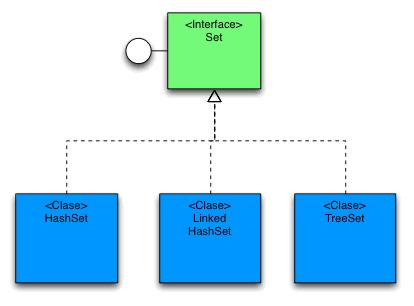
\includegraphics[scale=1]{interfazset.PNG}
\end{figure}

\section*{Interfaz Tablas Hash (Map) }
HashMap es una tabla en la que podemos insertar claves. Implementa el interface Map, lo cual nos permite utilizar los métodos relativos a los mapas. El rendimiento de las funciones básicas .get() y .put() es constante, ya que los elementos están dispersos en el mapa de forma concreta.
\subsection*{Métodos}
HashMap.containsKey(): Método que devuelve true si el mapa contiene la clave pasada como parámetro.

HashMap.entrySet(): Método que devuelve una vista del HashMap en formato colección. Cualquier modificación en la vista afecta directamente al contenido del HashMap.

HashMap.get(): Retorna el valor del HashMap para la clave pasada como parámetro.

HashMap.keySet(): Devuelve un conjunto con las claves que hay en el HashMap.

HashMap.put(): Inserta un par clave/valor en el mapa utilizando los valores pasados como parámetros.

HashMap.size(): Retorna el número de elemento clave/valor que tiene el HashMap.

HashMap.values(): Devuelve una colección con los valores del HashMap.

HashMap.clear(): Método que se usa para borrar y eliminar todos los elementos o asignaciones de un HashMap especificado.

HashMap.clone(): Método que se utiliza para devolver una copia superficial del mapa hash mencionado. Simplemente crea una copia del mapa.

HashMap.containsValue(): Este método se utiliza para verificar si un valor particular se asigna mediante una sola o más de una clave en el HashMap. Toma el valor como parámetro y devuelve verdadero si ese valor se asigna mediante alguna de las claves del mapa.

HashMap.isEmpty(): El método de la clase HashMap se usa para verificar el vacío del mapa. El método devuelve True si no hay un par de clave-valor o mapeo presente en el mapa de lo contrario False.

HashMap.putAll(): Es un método incorporado de la clase HashMap que se utiliza para la operación de copia. El método copia todos los elementos, es decir, las asignaciones, de un mapa a otro.

HashMap.remove(): Es un método incorporado de la clase HashMap y se utiliza para eliminar la asignación de cualquier clave particular del mapa. Básicamente, elimina los valores de cualquier clave en particular en el Mapa.

\section*{Uso de paquetes}
Los paquetes en Java (packages) son la forma en la que Java nos permite agrupar de alguna manera lógica los componentes de nuestra aplicación que estén relacionados entre sí.
Los paquetes permiten poner en su interior casi cualquier cosa como: clases, interfaces, archivos de texto, entre otros. De este modo, los paquetes en Java ayudan a darle una buena organización a la aplicación ya que permiten modularizar o categorizar las diferentes estructuras que componen nuestro software.
\subsection*{¿Cómo crear paquetes en Java?}
Para declarar un paquete en Java se hace uso de la palabra reservada "package" seguido de la "ruta" del paquete, como se muestra a continuación.
\begin{figure}[hbtp]
\centering
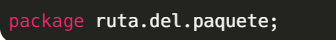
\includegraphics[scale=1]{1.PNG}
\end{figure}
\subsection*{Tips o prácticas para crear paquetes en Java}
\begin{enumerate}
\item El paquete en Java se declara antes que cualquier otra cosa.
\item Cada punto en la ruta del paquete es una nueva carpeta.
\item Si no se declara un paquete se utilizará el paquete por defecto.
\end{enumerate}
\bigskip Para usar clases de otros paquetes, no hay más que utilizar sentencias import, antes de la declaración de la clase.


Los ficheros .class pertenecientes a paquetes y subpaquetes deben estar organizados de forma adecuada para que tanto el compilador como la máquina virtual puedan utilizarlos.
Para ello, cada paquete se ubica en un directorio. Cada subpaquete se ubica en un directorio de nivel inferior, y así sucesivamente. Además, el nombre de cada directorio debe ser el del propio paquete.

A la hora de ejecutar una aplicación Java, hay que tener en cuenta algunas cosas. En primer lugar, hay que indicar el nombre completo de la clase a ejecutar.
\section*{Modificadores de acceso}
Los modificadores de acceso nos introducen al concepto de encapsulamiento. El encapsulamiento busca de alguna forma controlar el acceso a los datos que conforman un objeto o instancia, de este modo podríamos decir que una clase y por ende sus objetos que hacen uso de modificadores de acceso (especialmente privados) son objetos encapsulados.

Los modificadores de acceso permiten dar un nivel de seguridad mayor a nuestras aplicaciones restringiendo el acceso a diferentes atributos, métodos, constructores asegurándonos que el usuario deba seguir una "ruta" especificada por nosotros para acceder a la información.Es muy posible que nuestras aplicaciones vayan a ser usadas por otros programadores o usuarios con cierto nivel de experiencia; haciendo uso de los modificadores de acceso podremos asegurarnos de que un valor no será modificado incorrectamente por parte de otro programador o usuario. Generalmente el acceso a los atributos se consigue por medio de los métodos get y set, pues es estrictamente necesario que los atributos de una clase sean privados.

Nota: Siempre se recomienda que los atributos de una clase sean privados y por tanto cada atributo debe tener sus propios métodos get y set para obtener y establecer respectivamente el valor del atributo.

Nota 2: Siempre que se use una clase de otro paquete, se debe importar usando import. Cuando dos clases se encuentran en el mismo paquete no es necesario hacer el import pero esto no significa que se pueda acceder a sus componentes directamente.

\subsection*{Modificador de acceso private}
El modificador private en Java es el más restrictivo de todos, básicamente cualquier elemento de una clase que sea privado puede ser accedido únicamente por la misma clase por nada más. Es decir, si por ejemplo, un atributo es privado solo puede ser accedido por lo métodos o constructores de la misma clase. Ninguna otra clase sin importar la relación que tengan podrá tener acceso a ellos.
\begin{figure}[hbtp]
\centering
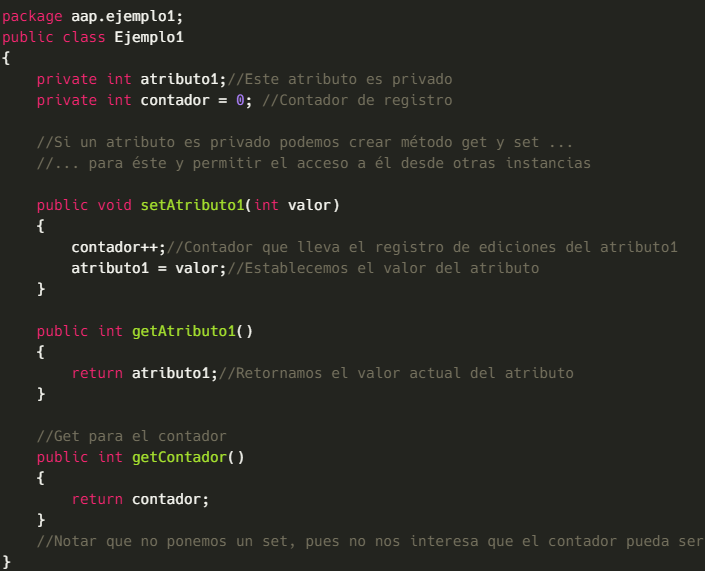
\includegraphics[scale=0.4]{2.PNG}
\end{figure}
\subsection*{El modificador por defecto (default)}
Java nos da la opción de no usar un modificador de acceso y al no hacerlo, el elemento tendrá un acceso conocido como defaulto acceso por defecto que permite que tanto la propia clase como las clases del mismo paquete accedan a dichos componentes (de aquí la importancia de declararle siempre un paquete a nuestras clases).
\begin{figure}[hbtp]
\centering
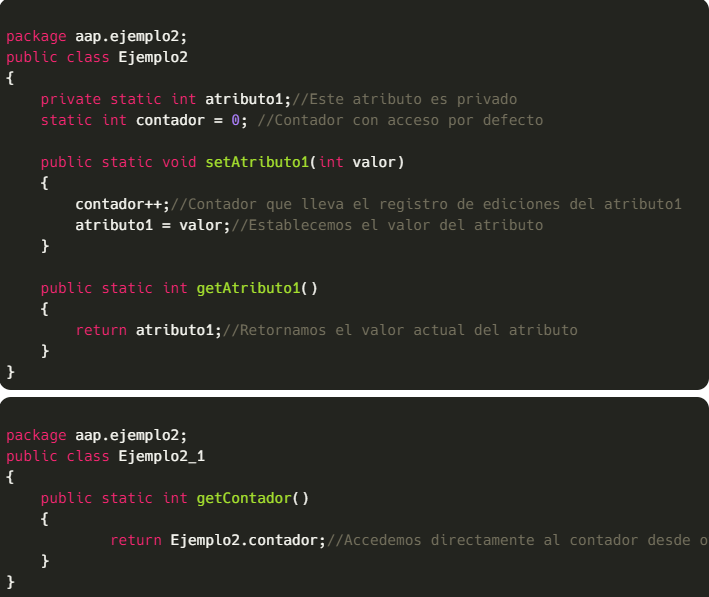
\includegraphics[scale=0.4]{3.PNG}
\end{figure}
\subsection*{Modificador de acceso protected}
El modificador de acceso protected nos permite acceso a los componentes con dicho modificador desde la misma clase, clases del mismo paquete y clases que hereden de ella (incluso en diferentes paquetes). 
\begin{figure}[hbtp]
\centering
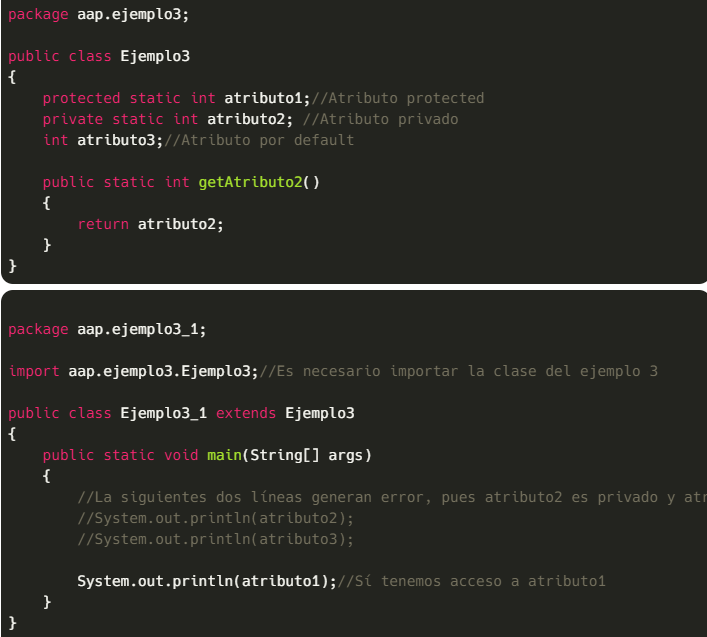
\includegraphics[scale=0.5]{4.PNG}
\end{figure}

\subsection*{Modificador public}
El modificador de acceso public es el más permisivo de todos, básicamente public es lo contrario a private en todos los aspectos (lógicamente), esto quiere decir que si un componente de una clase es public, tendremos acceso a él desde cualquier clase o instancia sin importar el paquete o procedencia de ésta.
\begin{figure}[hbtp]
\centering
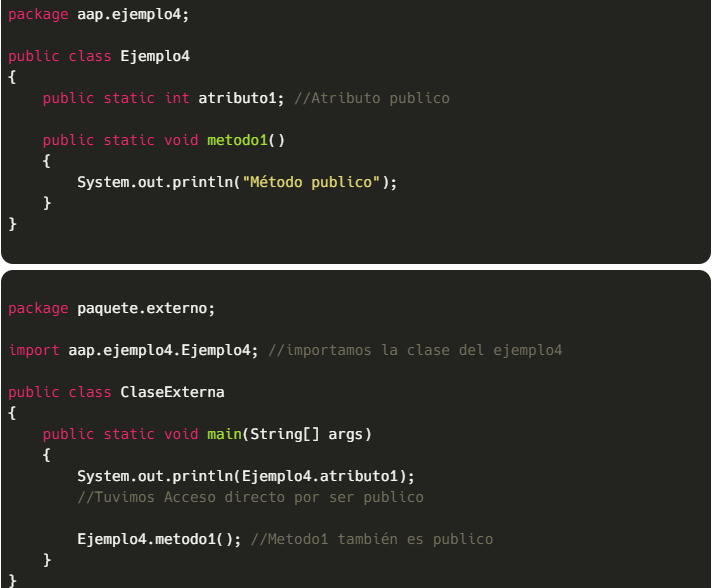
\includegraphics[scale=0.5]{5.PNG}
\end{figure}


A continuación, y ya para finalizar, se muestra una pequeña tabla que resume el funcionamiento de los modificadores de acceso en Java.
\begin{figure}[hbtp]
\centering
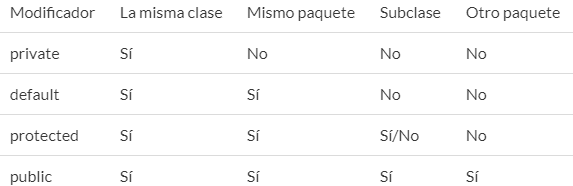
\includegraphics[scale=0.4]{6.PNG}
\end{figure}
\section*{Herencia y Polimorfismo}
La herencia es un pilar importante de OOP (Programación Orientada a Objetos). Es el mecanismo en Java por el cual una clase permite heredar las características (atributos y métodos) de otra clase. Aprenda más a continuación.

En el lenguaje de Java, una clase que se hereda se denomina superclase. La clase que hereda se llama subclase. Por lo tanto, una subclase es una versión especializada de una superclase. Hereda todas las variables y métodos definidos por la superclase y agrega sus propios elementos únicos.

Terminología importante

- Superclase: la clase cuyas características se heredan se conoce como superclase (o una clase base o una clase principal).

- Subclase: la clase que hereda la otra clase se conoce como subclase (o una clase derivada, clase extendida o clase hija). La subclase puede agregar sus propios campos y métodos además de los campos y métodos de la superclase.

- Reutilización: la herencia respalda el concepto de “reutilización”, es decir, cuando queremos crear una clase nueva y ya hay una clase que incluye parte del código que queremos, podemos derivar nuestra nueva clase de la clase existente. Al hacer esto, estamos reutilizando los campos/atributos y métodos de la clase existente.

\textbf{La palabra clave utilizada para la herencia es extends}
\subsection*{Tipos de herencia en Java}
\subsubsection*{Herencia única}
En la herencia única, las subclases heredan las características de solo una superclase. En la imagen a continuación, la clase A sirve como clase base para la clase derivada B.
\begin{figure}[hbtp]
\centering
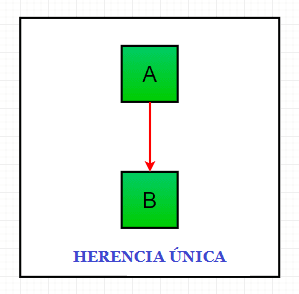
\includegraphics[scale=0.8]{herenciaunica.png}
\end{figure}

\subsubsection*{Herencia Multinivel}
En la herencia multinivel, una clase derivada heredará una clase base y, además, la clase derivada también actuará como la clase base de otra clase. En la imagen inferior, la clase A sirve como clase base para la clase derivada B, que a su vez sirve como clase base para la clase derivada C. En Java, una clase no puede acceder directamente a los miembros de los “abuelos”.
\begin{figure}[hbtp]
\centering
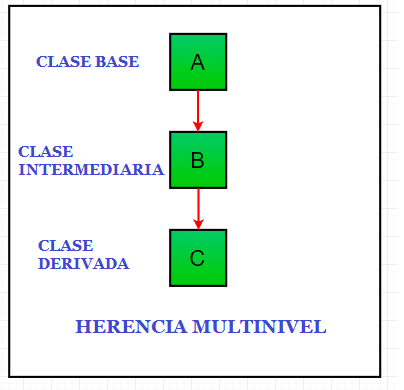
\includegraphics[scale=0.5]{herenciamultinivel.png}
\end{figure}

\subsubsection*{Herencia Jerárquica}
En la herencia jerárquica, una clase sirve como una superclase (clase base) para más de una subclase. En la imagen inferior, la clase A sirve como clase base para la clase derivada B, C y D.
\begin{figure}[hbtp]
\centering
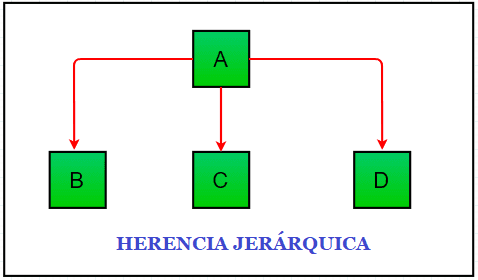
\includegraphics[scale=0.5]{herenciajerarquica.png}
\end{figure}

\subsubsection*{Herencia Múltiple (a través de interfaces)}
En Herencia múltiple, una clase puede tener más de una superclase y heredar características de todas las clases principales. Tenga en cuenta que Java no admite herencia múltiple con clases. En Java, podemos lograr herencia múltiple solo a través de Interfaces. En la imagen a continuación, la Clase C se deriva de la interfaz A y B.
\begin{figure}[hbtp]
\centering
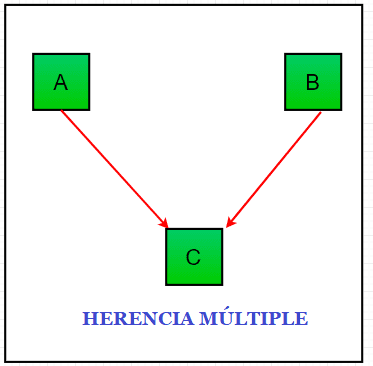
\includegraphics[scale=0.4]{herenciamultiple.png}
\end{figure}

\subsubsection{Herencia Híbrida (a través de Interfaces)}
Es una mezcla de dos o más de los tipos de herencia anteriores. Como Java no admite herencia múltiple con clases, la herencia híbrida tampoco es posible con clases. En Java, podemos lograr herencia híbrida solo a través de Interfaces.
\begin{figure}[hbtp]
\centering
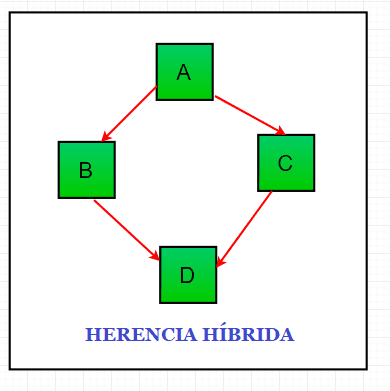
\includegraphics[scale=0.5]{herenciahibrida.png}
\end{figure}

\subsection*{Datos importantes acerca de la herencia en Java}
\begin{enumerate}
\item Superclase predeterminada: excepto la clase Object, que no tiene superclase, cada clase tiene una y solo una superclase directa (herencia única). En ausencia de cualquier otra superclase explícita, cada clase es implícitamente una subclase de la clase Object.
\item La superclase solo puede ser una: una superclase puede tener cualquier cantidad de subclases. Pero una subclase solo puede tener una superclase. Esto se debe a que Java no admite herencia múltiple con clases. Aunque con interfaces, la herencia múltiple es compatible con java.
\item Heredar constructores: una subclase hereda todos los miembros (campos, métodos y clases anidadas) de su superclase. Los constructores no son miembros, por lo que no son heredados por subclases, pero el constructor de la superclase puede invocarse desde la subclase.
\item Herencia de miembros privados: una subclase no hereda los miembros privados de su clase principal. Sin embargo, si la superclase tiene métodos públicos o protegidos (como getters y setters) para acceder a sus campos privados, estos también pueden ser utilizados por la subclase.
\end{enumerate}
\subsection*{Polimorfismo}
Polimorfismo es la capacidad de un objeto de adquirir varias formas. El uso más común de polimorfismo en programación orientada a objetos se da cuando se utiliza la referencia de una clase padre, para referirse al objeto de la clase hijo.

Cualquier objeto java que pueda pasar más de un test "ES-UN" es considerado polimórfico. En Java, todos los objetos son polimórficos ya que cualquier objeto pasaría un test "ES-UN" dado que son de su propio tipo, además del de la clase Object.

Es importante saber que la única manera de acceder a un objeto es a través de una variable de referencia. La variable de referencia sólo puede ser de un tipo. Una vez declarado el tipo de la variable de referencia, no se puede cambiar.

La variable de referencia puede ser reasignada a otros objetos, siempre y cuando no haya sido declarada "final". El tipo de la variable de referencia, determina los métodos que podrán ser llamados sobre el objeto.

Una variable de referencia puede hacer referencia a cualquier objeto o cualquier subtipo de su propio tipo.\begin{figure}[hbtp]
\centering
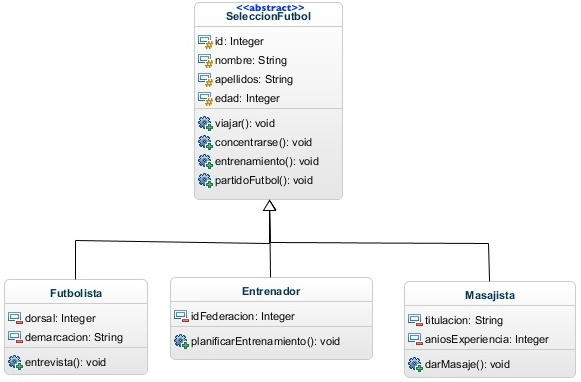
\includegraphics[scale=0.5]{PolimorfismoFutbol-diag.jpg}
\end{figure}
\section*{Clases Abstractas e Interfaces}
\subsection*{Clases Abstractas }
Una clase que declara la existencia de métodos pero no la implementación de dichos métodos (o sea, las llaves { } y las sentencias entre ellas), se considera una clase abstracta. 

Una clase abstracta puede contener métodos no-abstractos pero al menos uno de los métodos debe ser declarado abstracto. 

Para declarar una clase o un metodo como abstractos, se utiliza la palabra reservada abstract. 

Una clase abstracta no se puede instanciar pero si se puede heredar y las clases hijas serán las encargadas de agregar la funcionalidad a los métodos abstractos. Si no lo hacen así, las clases hijas deben ser también abstractas.
\subsection*{Interfaces }
Una interface es una variante de una clase abstracta con la condición de que todos sus métodos deben ser asbtractos. Si la interface va a tener atributos, éstos deben llevar las palabras reservadas static final y con un valor inicial ya que funcionan como constantes por lo que, por convención, su nombre va en mayúsculas. 

Una clase implementa una o más interfaces (separadas con comas ",") con la palabra reservada implements. Con el uso de interfaces se puede "simular" la herencia múltiple que Java no soporta. 

La clase que implementa una interface tiene dos opciones: 

1) Implementar todos los métodos de la interface. 

2) Implementar sólo algunos de los métodos de la interface pero esa clase debe ser una clase abstracta (debe declararse con la palabra abstract).

\begin{figure}[hbtp]
\centering
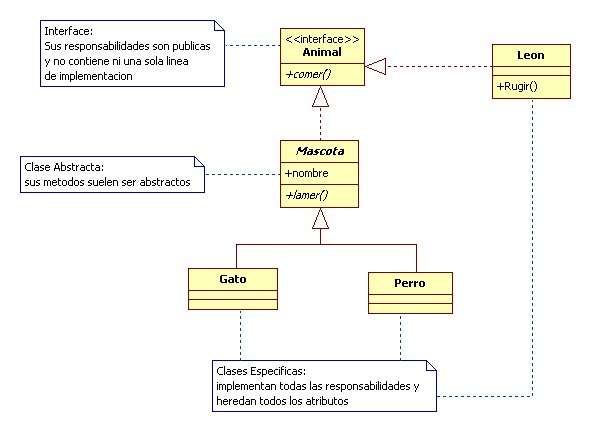
\includegraphics[scale=0.5]{Clases-Abstractas-e-Interfaces.jpg}
\end{figure}
\section*{Uso de excepciones }
Una ventaja principal del manejo de excepciones es que automatiza gran parte del código de manejo de errores que previamente debía ingresarse “a mano” en cualquier programa grande. Por ejemplo, en algunos lenguajes de computadora más antiguos, los códigos de error se devuelven cuando falla un método, y estos valores se deben verificar manualmente, cada vez que se llama al método. Este enfoque es tedioso y propenso a errores.

El manejo de excepciones agiliza el manejo de errores al permitir que tu programa defina un bloque de código, llamado manejador de excepción, que se ejecuta automáticamente cuando ocurre un error. No es necesario verificar manualmente el éxito o el fracaso de cada operación específica o llamada a un método. Si se produce un error, será procesado por el manejador de excepciones.

\subsection*{Fundamentos de manejo de excepciones}
El manejo de excepciones Java se gestiona a través de cinco palabras clave: try, catch, throw, throws,
y finally. Forman un subsistema interrelacionado en el que el uso de uno implica el uso de otro. . En resumen, así es como funcionan.

Las declaraciones de programa que desea supervisar para excepciones están contenidas dentro de un bloque try. Si se produce una excepción dentro del bloque try, se lanza. Tu código puede atrapar esta excepción usando catch y manejarlo de una manera racional. Las excepciones generadas por el sistema son lanzadas automáticamente por el sistema de tiempo de ejecución de Java. Para lanzar manualmente una excepción, use la palabra clave throw. En algunos casos, una excepción arrojada por un método debe ser especificada como tal por una cláusula throws. Cualquier código que debe ejecutarse al salir de un bloque try se coloca en un bloque finally.

\subsection*{Jerarquía de excepciones}
En Java, todas las excepciones están representadas por clases. Todas las clases de excepción se derivan de una clase llamada Throwable. Por lo tanto, cuando se produce una excepción en un programa, se genera un objeto de algún tipo de clase de excepción.

Hay dos subclases directas de Throwable: Exception y Error:

\begin{enumerate}
\item Las excepciones de tipo Error están relacionadas con errores que ocurren en la Máquina Virtual de Java y no en tu programa. Este tipo de excepciones escapan a su control y, por lo general, tu programa no se ocupará de ellas.
\item Los errores que resultan de la actividad del programa están representados por subclases de Exception. Por ejemplo, dividir por cero, límite de matriz y errores de archivo caen en esta categoría. En general, tu programa debe manejar excepciones de estos tipos. Una subclase importante de Exception es RuntimeException, que se usa para representar varios tipos comunes de errores en tiempo de ejecución.
\end{enumerate}
\begin{figure}[hbtp]
\centering
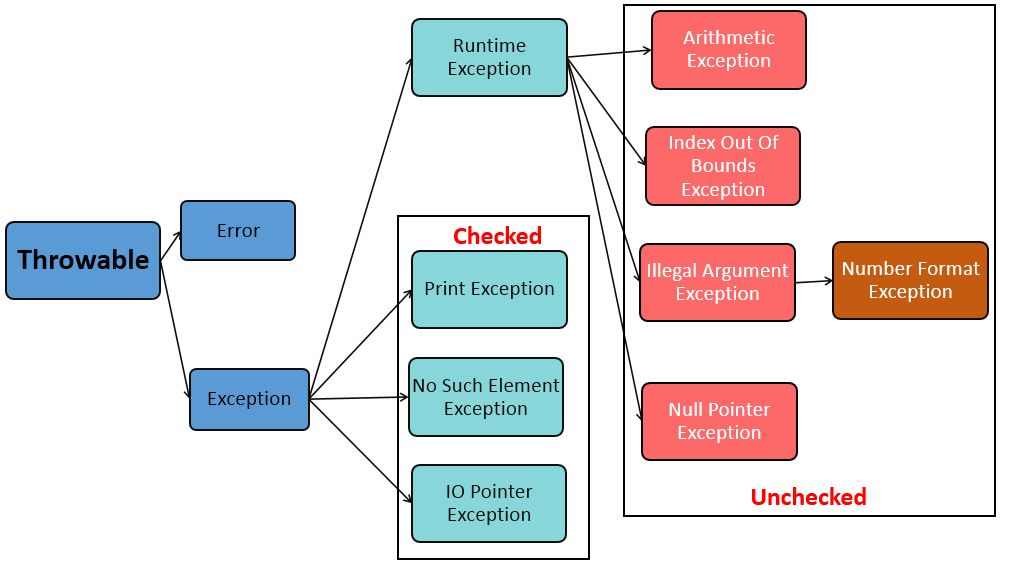
\includegraphics[scale=0.5]{ExcepcionesCheckedUnchecked.png}
\end{figure}

\section*{Manejo de archivos}
\subsection*{Los archivos desde Java}
En Java, los distintos tipos de ficheros se diferencian por las clases que usaremos para representarlos y manipularlos. Como las clases que usaremos pertenecen a la biblioteca estándar del lenguaje, su uso es algo más complejo que las de las clases de la ACM, ya que su diseño se ha realizado pensando en su uso industrial. Las clases que usaremos para el tratamiento de ficheros están ubicadas en el paquete java.io por lo que deben ser importadas. Además, el código que trabaja con archivos ha de considerar que muchas cosas pueden ir mal cuando se trabaja con ellos: el archivo puede estar corrupto, alguien ha desconectado el pendrive a medio ejecutar del programa, es un disco en red y ésta ha caído, o no tiene más espacio para almacenar información, etc.  Es por ello que, aunque de forma breve, deberemos introducir el mecanismo estándar en Java para tratar con los errores que pueden darse en nuestro programa: las excepciones.

Java proporciona un numero amplio de clases, muy útiles para trabajar sobre ficheros a través del paquete Java.io. Para ver un ejemplo del poder de este paquete vamos a crear una pequeña clase que nos permita crear y eliminar  ficheros además que posibilite buscar, modificar, y eliminar registros dentro del archivo.

Comencemos por crear el fichero, pero primero debemos hacer uso de la clase File, que es la que nos proporciona información acerca del archivo: 
\begin{figure}[hbtp]
\centering
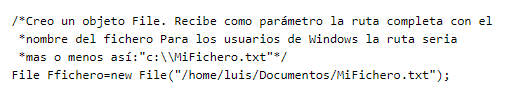
\includegraphics[scale=1]{archivo.PNG}
\end{figure}

\textbf{Clases para flujos de entrada }

Se utilizan para leer datos de una fuente de entrada (archivo, cadena o memoria)

\textbf{Flujo de bytes:} InputStream, BufferedInputstream, DataInputStream, FileInputStream

\textbf{Flujo de caracteres:} Reader, BufferReader, FileReader
\bigskip 

\textbf{Clases para flujo de salida}
Son las homologas a las clases de flujo de entrada y se utilizan para enviar flujos de datos a dispositivos de salida.

\textbf{Flujo de bytes:} OutputStream, PrintStream y FileOutputStream

\textbf{Flujo de caracteres:} Writer, PrintWriter, FileWriter

\textbf{Clases de Archivo:}File y RandomAccesFile (mayor control sobre los archivos)

\section*{Interfaces gráficas de usuario}
La interfaz de usuario es la parte del programa que permite al usuario interaccionar con él. 

La API de Java proporciona una biblioteca de clases para el desarrollo de Interfaces gráficas de usuario (en realidad son dos). 

La biblioteca proporciona un conjunto de herramientas para la construcción de interfaces gráficas que tienen una apariencia y se comportan de forma semejante en todas las plataformas en las que se ejecuten.
 La estructura básica de la biblioteca gira en torno a componentes y contenedores. Los contenedores contienen componentes y son componentes a su vez, de forma que los eventos pueden tratarse tanto en contenedores como en componentes. 
 
La API está constituida por clases, interfaces y derivaciones. 
AWT y Swing

\begin{figure}[hbtp]
\caption{Algunos componentes de AWT}
\centering
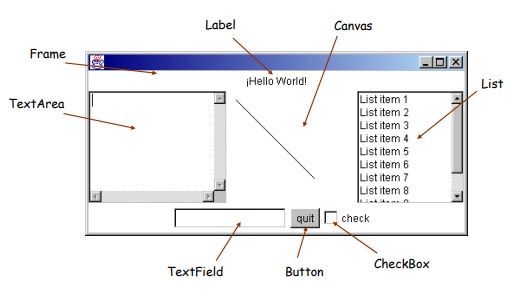
\includegraphics[scale=1]{AWT.PNG}
\end{figure}

\begin{figure}[hbtp]
\caption{Algunos componentes de Swing}
\centering
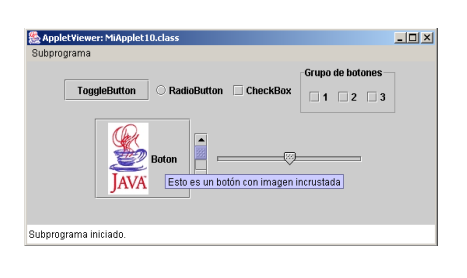
\includegraphics[scale=1]{SWING.PNG}
\end{figure}

\subsection*{Swing}
Paquete de Java para la generación del GUI en aplicaciones reales de gran tamaño. Disponible como paquete externo en Java 1.1 e integrado desde Java 1.2. 

Es una de las API de JFC (Java Foundation Classes): AWT, Java 2D, Accessibility, Drag and Drop, Swing, ... 

Escrito totalmente en Java. No reemplaza a AWT. Se apoya sobre AWT y añade JComponents.

Utiliza el modelo de eventos de Java 1.1. Elección entre diferentes aspectos (look and feel). 

Arquitectura Model-View-Controller (MVC). 

Nuevos componentes (árboles, tablas, frames internos, iconos, bordes, tooltips, beans, etcétera).
\subsection*{Jerarquía de clases para las GUI}

\begin{figure}[hbtp]
\caption{Jerarquía de clases para las GUI}
\centering
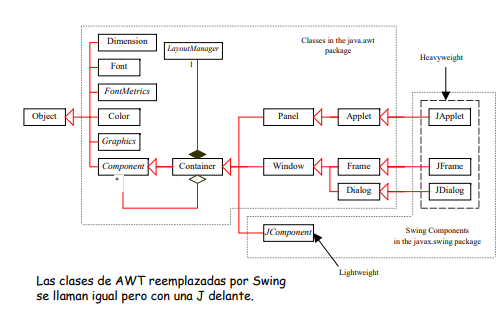
\includegraphics[scale=1]{Jerarquia.PNG}
\end{figure}

\begin{itemize}
\item Component: superclase de todas las clases de interfaz gráfica. 
\item Container: para agrupar componentes. 
\item JComponent: superclase de todos los componentes de Swing que se dibujan directamente en los lienzos (canvas). Sus subclases son los elementos básicos de la GUI. 
\item JFrame: ventana que no está contenida en otras ventanas. 
\item JDialog: cuadro de diálogo. 
\item JApplet: subclase de Applet para crear applets tipo Swing. 
\item JPanel: contenedor invisible que mantiene componentes de interfaz y que se puede anidar, colocándose en otros paneles o en ventanas. También sirve de lienzo. 
\item Graphics: clase abstracta que proporciona contextos gráficos donde dibujar cadenas de texto, líneas y otras formas sencillas.
\item Color: color de los componentes gráficos. 
\item Font: aspecto de los caracteres. 
\item FontMetrics: clase abstracta para propiedades de las fuentes.
\end{itemize}

\textbf{Categorías de clases: }
\begin{enumerate}
\item Contenedores: JFrame, JApplet, JWindow, JDialog 
\item Componentes intermedios: JPanel, JScrollPane 
\item Componentes: JLabel, JBbutton, JTextField, JTextArea, ... 
\item Clases de soporte: Graphics, Color, Font, ...
\end{enumerate}

\begin{figure}[hbtp]
\caption{Jerarquía de clases para las GUI: JComponent}
\centering
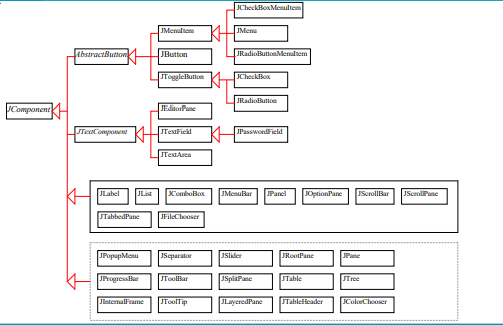
\includegraphics[scale=0.8]{JComponent.PNG}
\end{figure}

\begin{figure}[hbtp]
\caption{Jerarquía de clases para las GUI: AWT}
\centering
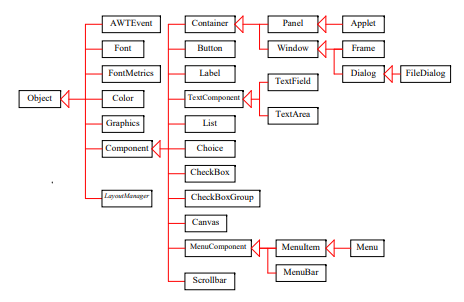
\includegraphics[scale=0.8]{Jerarquia AWT.PNG}
\end{figure}

\subsection*{Uso de imagenes}
No es necesario que conviertas la imagen a .ico, Java lo hará por nosotros, para el JFrame. Para otros componentes sera necesario que adaptes la imagen a tus necesidades, ya que sino aparecerá con su tamaño real.

La clase con la que manejaremos las imágenes es con ImageIcon(String) donde le pasaremos un String con la ruta de la imagen. En aquellos elementos que puedan contener un icono, suelen tener un constructor que incluye un parámetro de la clase Icon o Image.

Lo ideal es que cuando hacemos una aplicación que use imágenes, creamos una carpeta en el proyecto que contenga todas las imágenes usadas. Es importante saber que si queremos usar una ruta relativa, esta empieza desde la raíz del proyecto, no de la carpeta src.



\subsection*{Uso de tablas en Java}
Para usar tablas en Java podemos apoyarnos de la herramienta “JTable”, el cual es un componente visual el cual nos permite dibujar una tabla con filas/columnas donde podemos poner y modificar datos a nuestro gusto.

Como usa una serie de componentes modelo-vista, los datos que son usados dentro de la tabla son modificados de tal forma que el usuario del programa que usa ésta solo podrá ver los contenidos que se necesiten ver, mientras que dentro del código es donde se realizan los diversos cambios. Por eso el nombre “modelo-vista”.

Es recomendado que para usar una tabla en java, primero sea creada una instancia de “DefaultTableModel” y luego un “JTable” donde se le pasa como modelo el constructor. Esto es porque “DefaultTableModel” tiene todos los métodos necesarios para que la modificación de datos dentro de la tabla pueda ser realizada de forma eficiente.

De igual forma es recomendado que la clase que use la tabla implemente la interface “TableModel”, ya que esta permite al programador redefinir múltiples métodos a su gusto.

Por ejemplo, si queremos acceder a una imagen en la carpeta imágenes de nuestro proyecto, le pasaremos “imagenes \ imagen.jpg”,lo recomendable es usar la contante separator de la clase File, quedándose así “imagenes”+File.separator+”imagen.jpg”.

Le podemos cambiar en cualquier momento el icono a nuestro JFrame, con el método setIconImagen(“objeto IconImage”.getImage()). Para los demás componentes, usaremos el método setIcon(Icon), le podemos pasar un objeto de ImageIcon.

\section*{Organización del programa}
Nuestro proyecto queda organizado en 6 paquetes el cual el default es el paquete principal. Para que estos paquetes puedan usarse de forma adecuada serán importados a los paquetes correspondientes para su dicho uso. Trabajamos en varios paquetes para que nuestra información de vea de una forma más clara y organizada.

\begin{figure}[hbtp]
\centering
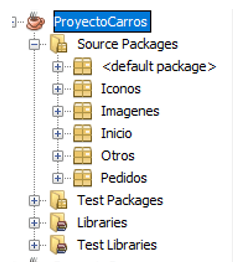
\includegraphics[scale=0.5]{OP1.PNG}
\end{figure}


En el primer paquete veremos el implemento de nuestras varias interfaces graficas que serán llamadas mediante llamadas de objetos en cada interface, la clase ProyectoCarros.java será nuestra clase principal que ejecutará a todas las demás. 

\begin{figure}[hbtp]
\centering
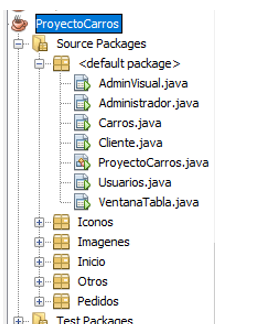
\includegraphics[scale=0.5]{OP2.PNG}
\end{figure}

Los paquetes iconos e imágenes tienen las imágenes correspondientes a las interfaces que ocuparan nuestras interfaces.

El paquete inicio y otros, son paquetes que serán usados en nuestra interface llamada Carros que serán llamadas mientras el botón Ingresar.

Nota: Para llamar las clases correspondientes, lo único que teníamos que hacer es darle clic al botón y esta nos enviaría a una ventana para meter ahí el objeto y entonces poder llamarlos, así funciona con todos nuestros botones.

Por ejemplo, a dar clic en Ingresar datos, creábamos el objeto para poder hacer uso de este, acción que se repetía con los demás botones.

\begin{figure}[hbtp]
\centering
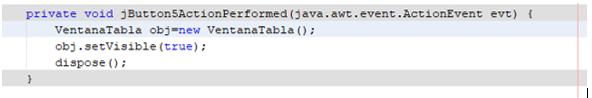
\includegraphics[scale=1]{OP3.PNG}
\end{figure}

En la clase pedidos pusimos el código general, donde se incluían casi todos los temas vistos a lo largo del semestre, ahí fue donde hicimos uso de la interface, esto fue porque no necesariamente un carro debe ser igual a otros y cada uno de ellos debería implementar ciertas características, tal es el caso de la clase camioneta y la clase vagoneta.

Ahí también hicimos el uso le lectura y escritura para guardar los datos archivados (eso también lo hicimos en la parte de Ingresar datos mediante el uso de tablas).

\begin{figure}[hbtp]
\centering
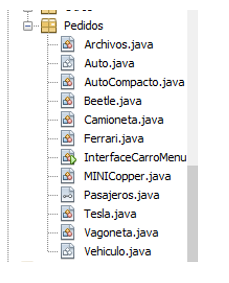
\includegraphics[scale=0.8]{OP4.PNG}
\end{figure}

Para el botón ingresar, decidimos hacer el uso de tablas, ya que era mucho más fácil guardar información, editar y eliminar como se verá en nuestro proyecto en su ejecución.

\begin{figure}[hbtp]
\centering
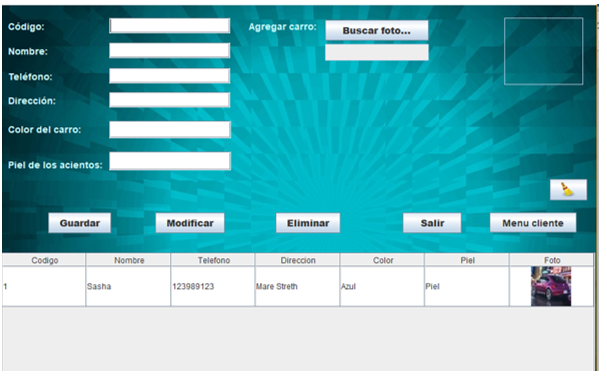
\includegraphics[scale=0.8]{OP5.PNG}
\end{figure}


\section*{Conclusiones}
\textbf{Félix Flores Paul Jaime.}
\bigskip 

Al hacer este último proyecto decidimos que íbamos hacer el proyecto de la agencia automotriz, ya que teníamos una práctica similar al proyecto, lo único que debíamos hacer es pequeñas modificaciones a nuestro programa, así del mismo modo, investigar sobre las interfaces gráficas.
\medskip 

Me encanto hacer el uso del implemento de interfaces, ya que me encanta ver algo visual y no hacer un código en computadora y como se me da el crear cosas, creo que hice un buen trabajo al investigar cosas acerca de interface, traté de agarrar ciertas cosas de tutoriales de YouTube y al final juntarlo todo de acuerdo a la funcionalidad de nuestro proyecto. 
\medskip 

Creo que lo más complicado a la hora de armar el programa, fue que teníamos que tratar de organizarlo correctamente en las carpetas, ya que si hacíamos algo mal podía tronar el programa. Lo tratamos de solucionar haciendo, poner un programa y después otro y así compilarlo de poco a poco y así yéndonos por todos y no tratar de compilar todo de un jalón y terminar con muchos errores.
\medskip 

Otra cosa que cabe mencionar fue que englobamos todo lo que vimos a lo largo del semestre, ya que como vimos en nuestro proyecto nuestra   clase perro había evolucionado por completo y así convirtiéndose en un programa mucho más completo. Me siento muy contento con el proyecto, ya que logramos implementar todo lo que vimos, así como hacer una buena interfaz, quizás si hubiéramos tenido más tiempo hubiéramos puesto más cosas, pero creo que logramos de cumplir el objetivo.
\bigskip 

\textbf{Sergio Ángel Hernández Luis}
\bigskip 

Durante el desarrollo de este proyecto se vio la implementación de los diferentes conceptos que se han visto durante el curso, además de buscar otros tipos de conceptos para poder desarrollar el problema planteado.
\medskip 

Uno de los aspectos que más se tuvo que investigar fue la implementación de las interfaces graficas ya que fue un concepto nuevo y con ello aprendimos como darle algo más estético a nuestros proyectos dentro de java, por lo que su implementación fue de los aspectos más interesantes del proyecto. Ya que ahora no solo trabajamos con código y una consola, sino que ahora podíamos darle la apariencia que mejor nos pareciera.
\medskip 

Otra parte que se complico fue integrar el manejo de archivos, ya que al usar las interfaces graficas se tenía que buscar cómo implementarlos sin modificar demasiado el código base, lo que se pensó primero fue crear un arrayList de los objetos y posteriormente guardarlos en un archivo de objetos, lo cual se logró. Sin embargo, al momento de quererlos leer para poder mostrarlos no se hacia el proceso de lectura. Por lo que se decidió usar archivos de texto plano.
\medskip 

En general considero que los objetivos planteados para este proyecto fueron cumplidos ya que ahora se conoce el funcionamiento de otras herramientas que pueden ayudar en el desarrollo de aplicaciones del mundo real.
\bigskip 

\textbf{Ricardo Alonso Velasco Vanegas}
\bigskip 

En conclusión este ha sido uno de los proyectos más complicados que he realizado en todos mis cursos de programación con todos los demás profes. En el proyecto final se usaron tantos conceptos distintos que el lograr que estos funcionaran correctamente fue todo un reto. En particular se encontraron problemas a la hora de utilizar paquetes para las imágenes y cuando se colocó la interfaz gráfica, pero con esfuerzo constante esos problemas fueron resueltos.
\medskip 

De igual forma en el transcurso del proyecto se nos ocurrió la idea de usar tablas para guardar y editar la información de manera más sencilla dentro de archivos externos, ya que es un tema que me resulta personalmente difícil.

\section{Bibliografia}

\bibliography{Reporte}
Eric S. Roberts. The Art and Science of Java (Preliminary Draft)

Snajdleder, P (2007). Algoritmos a Fondo: - Con implementaciones en c y java. Editorial Ink.

Sunggu Lee (2000). Dise~no de Computadoras y Otros Dispositivos Digitales Complejos. Prentice
Hall.

Luis Joyanes Aguilar, Ignacio ZahoneroMartìnez,Programaciòn en Java 2: Algoritmos, Estructuras de Datos y Programaciòn Orientada a Objetos, Madrid, McGraw Hill Interamericana. 

Deitel , Harvey. DeitelPaul(2004): Como programar en JAVA. Quinta Edición, Pearson educación 

Sierra, K., Bates, B. Head First Java, O’Reilly, Sebastopol, CA, 2nd Edition, 2005

Manual de prácticas del laboratorio de Programación orientada a objetos


\end{document}